

\chapter{Anexos}\label{chap:fich-act}

Fichas que se entregarán ás alumnas e alumnos para a realización de actividades.
\begin{itemize}
  \item Ficha da actividade 0.
  \item Problemas propostos de Mediatrices e Bisectrices.
  \item Exame Elementos Básicos de Xeometría.
  \item Imaxes empregadas para traballar os puntos notables dun triángulo.
  \item Problemas propostos do Teorema de Pitágoras.
  \item Preguntas do Trivial da Actividade 13
  \item Exame Polígonos.
  \item Entradas blogue.
\end{itemize}
\newpage


\includepdf[pages=-,angle=270,scale=0.8,offset=0mm -17mm,frame, pagecommand={\section{Ficha da Actividade 0}\label{fich:act0}}]{pdf/act0x2.pdf}

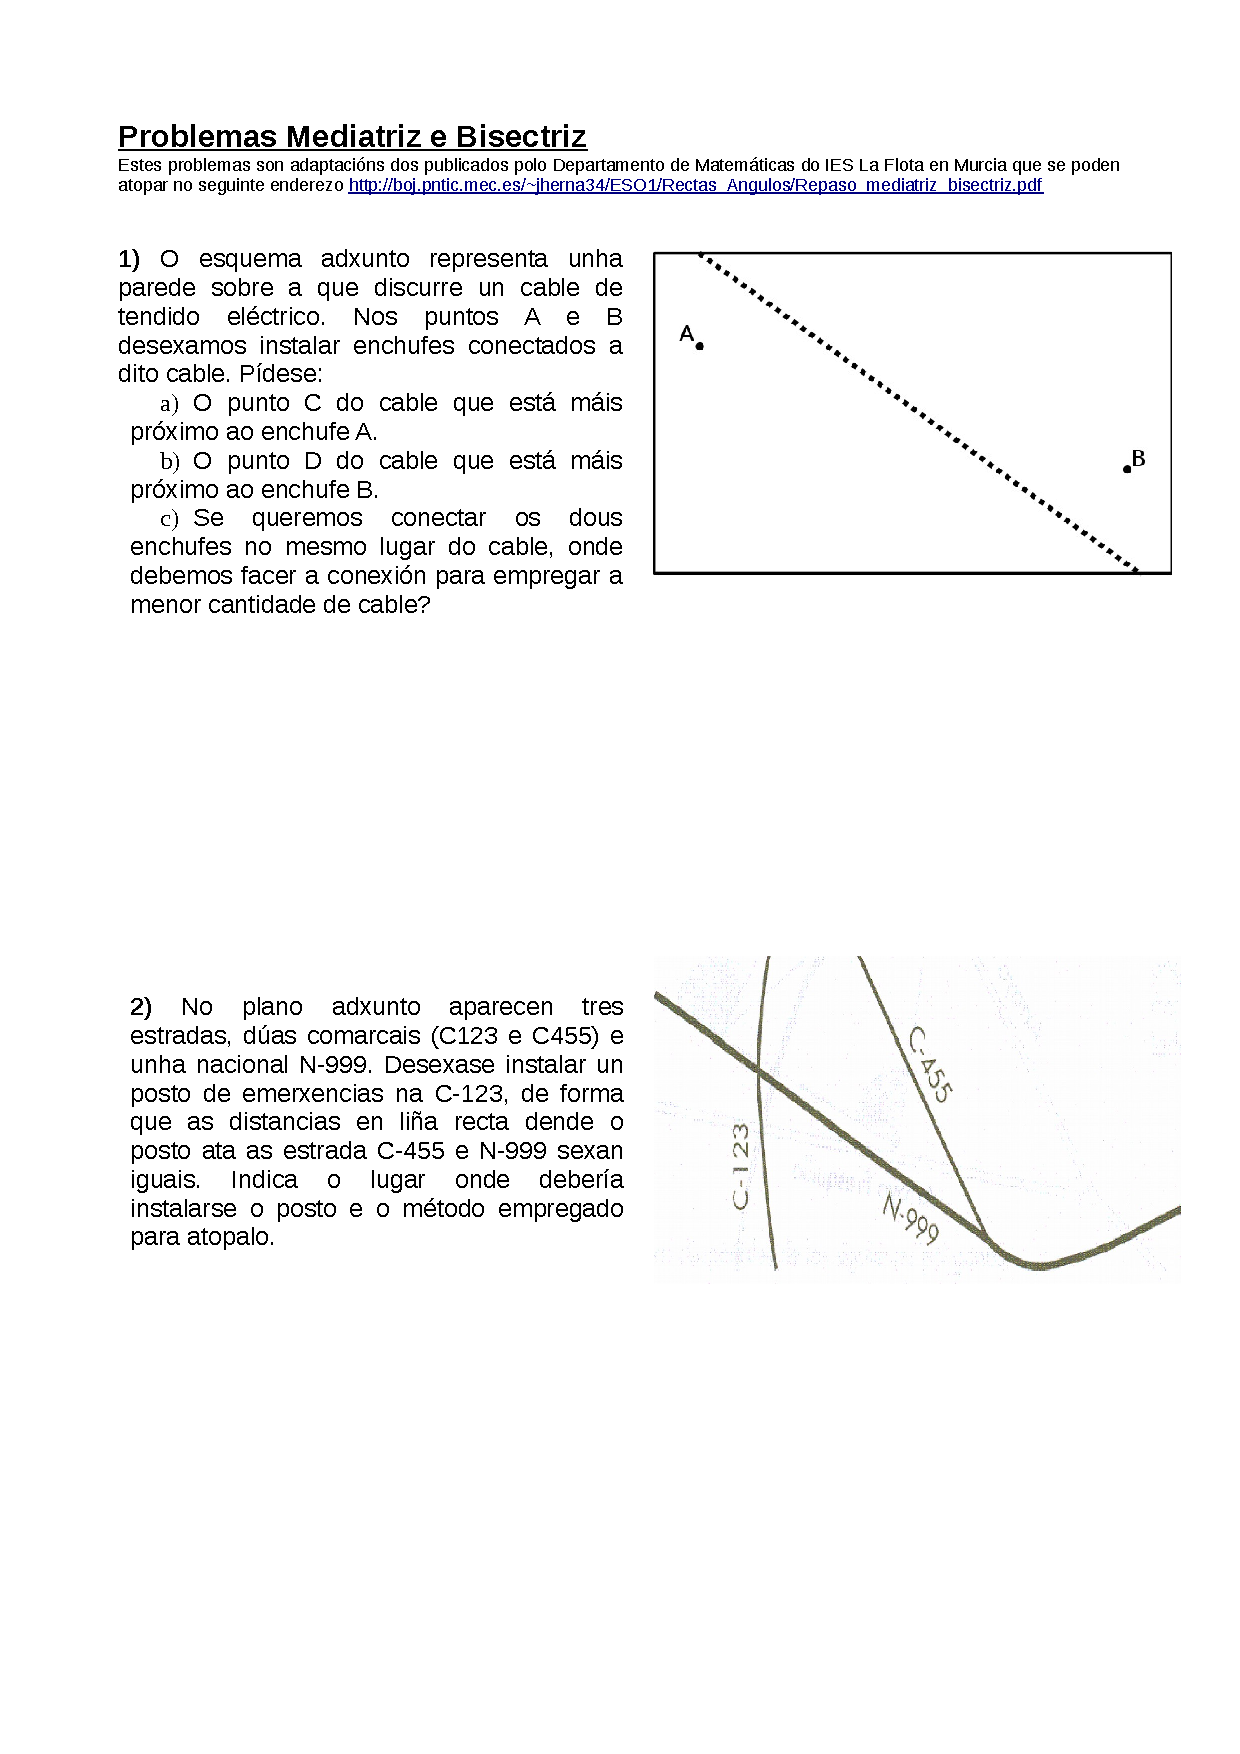
\includepdf[pages=1,scale=0.8,offset=0mm -17mm, frame,pagecommand={\section{Problemas propostos de Mediatrices e Bisectrices}\label{fich:mediatriz}}]{pdf/mediatriz.pdf}
\includepdf[pages=2,scale=0.8,offset=0mm -17mm, frame,pagecommand={}]{pdf/mediatriz.pdf}

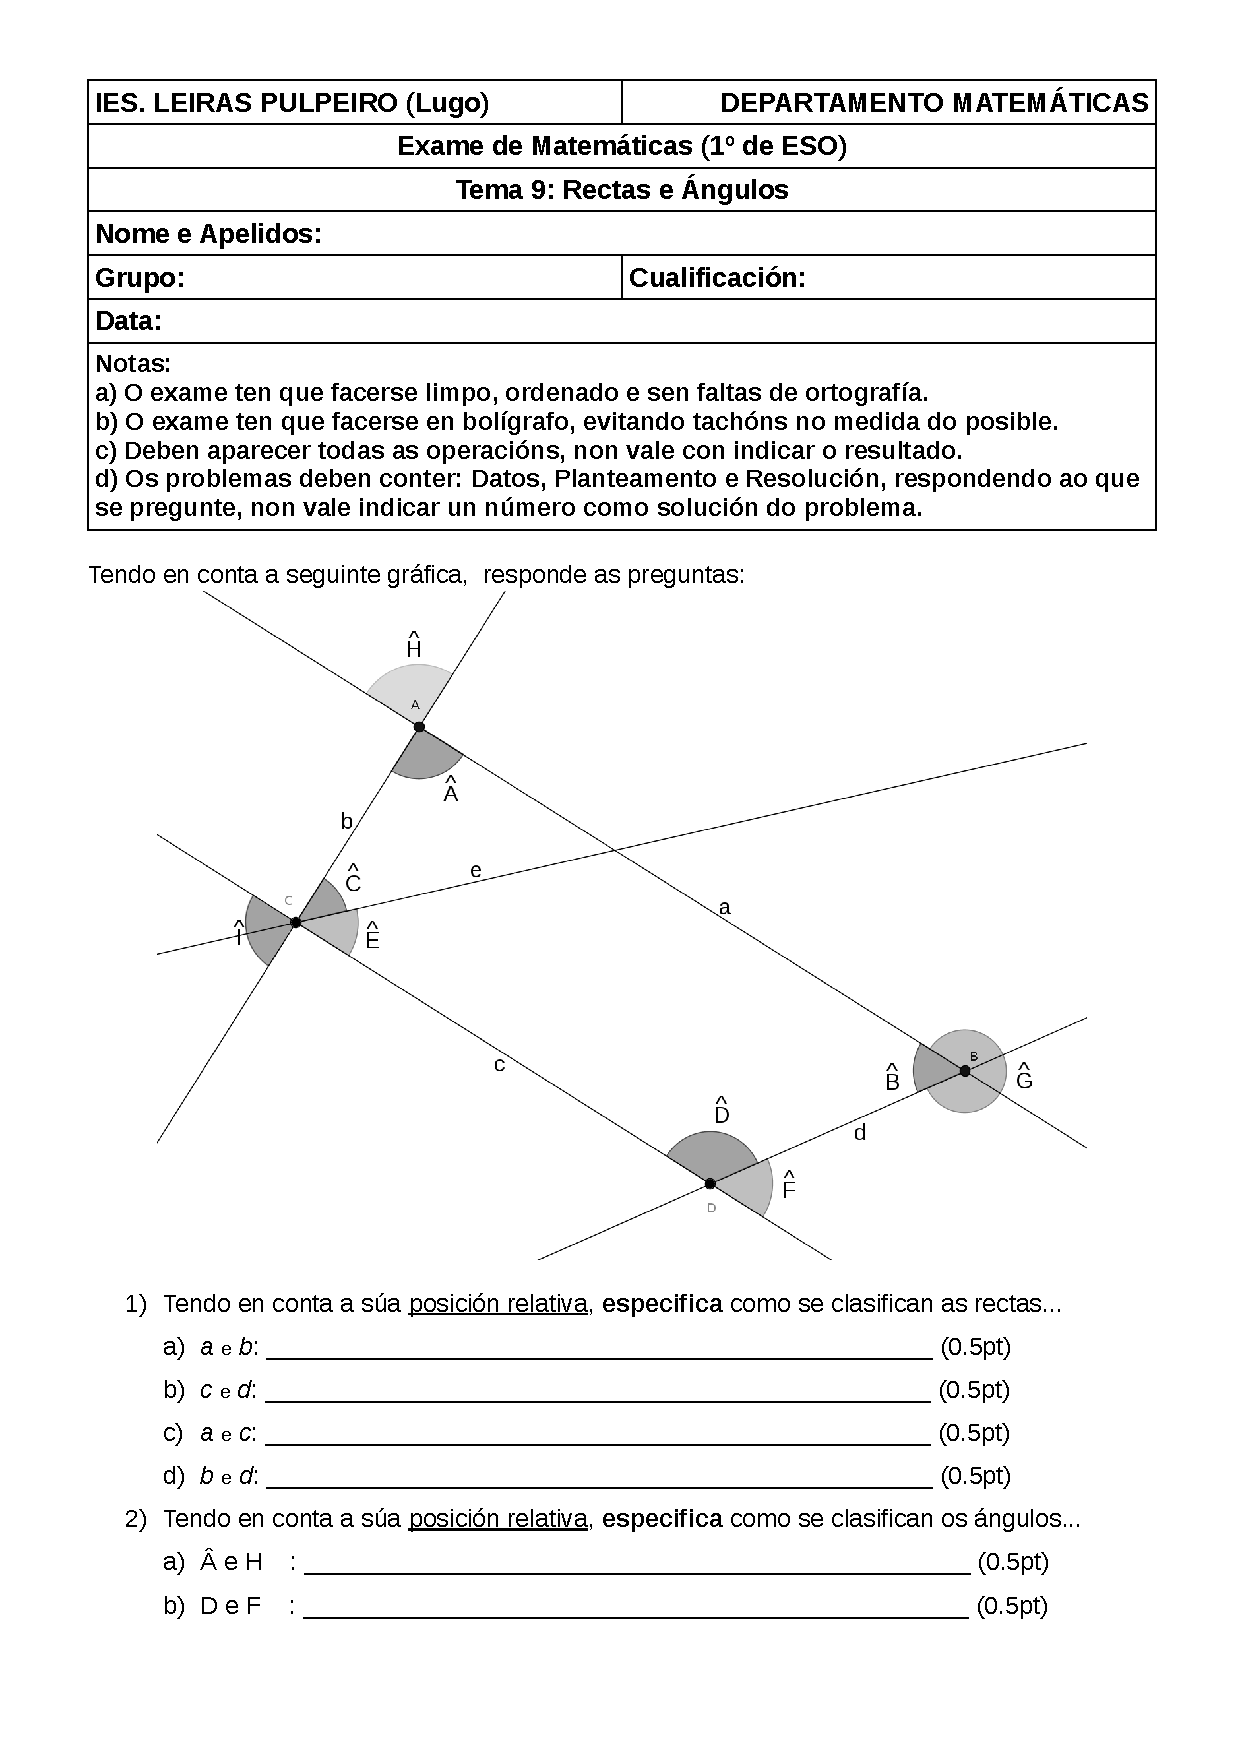
\includepdf[pages=1,scale=0.8,offset=0mm -17mm, frame,pagecommand={\section{Exame Elementos Básicos de Xeometría}\label{fich:ex1a}}]{pdf/exame1.pdf}
\includepdf[pages=2,scale=0.8,offset=0mm -17mm, frame,pagecommand={}]{pdf/exame1.pdf}

\section{Imaxes empregadas para traballar os puntos notables dun triángulo}\label{fich:notables}
\begin{figure}[h!]
  \centering
  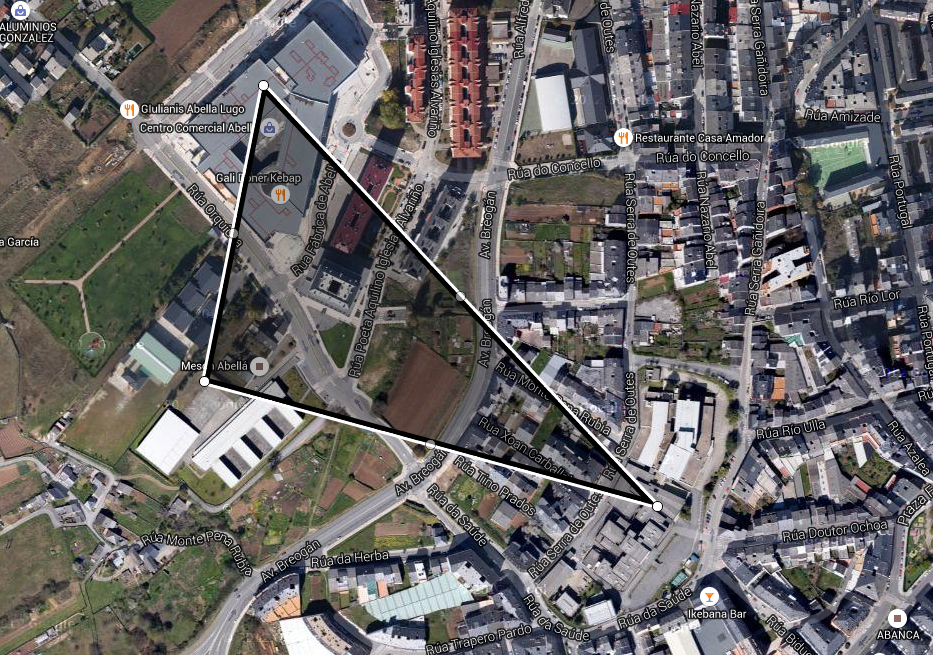
\includegraphics[width=0.8\textwidth]{img/circuncentro.png}
  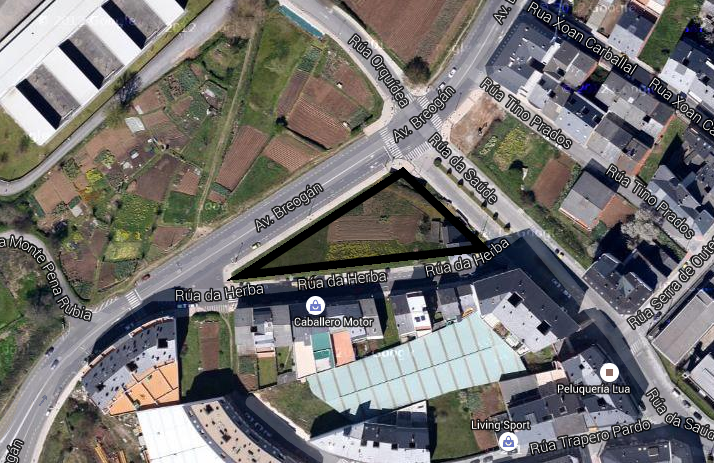
\includegraphics[width=0.8\textwidth]{img/incentro.png}
  \caption{Imaxes empregadas para explicar o circuncentro e incentro}\label{fig:act12-1}\label{fig:act12-2}
\end{figure}
\newpage


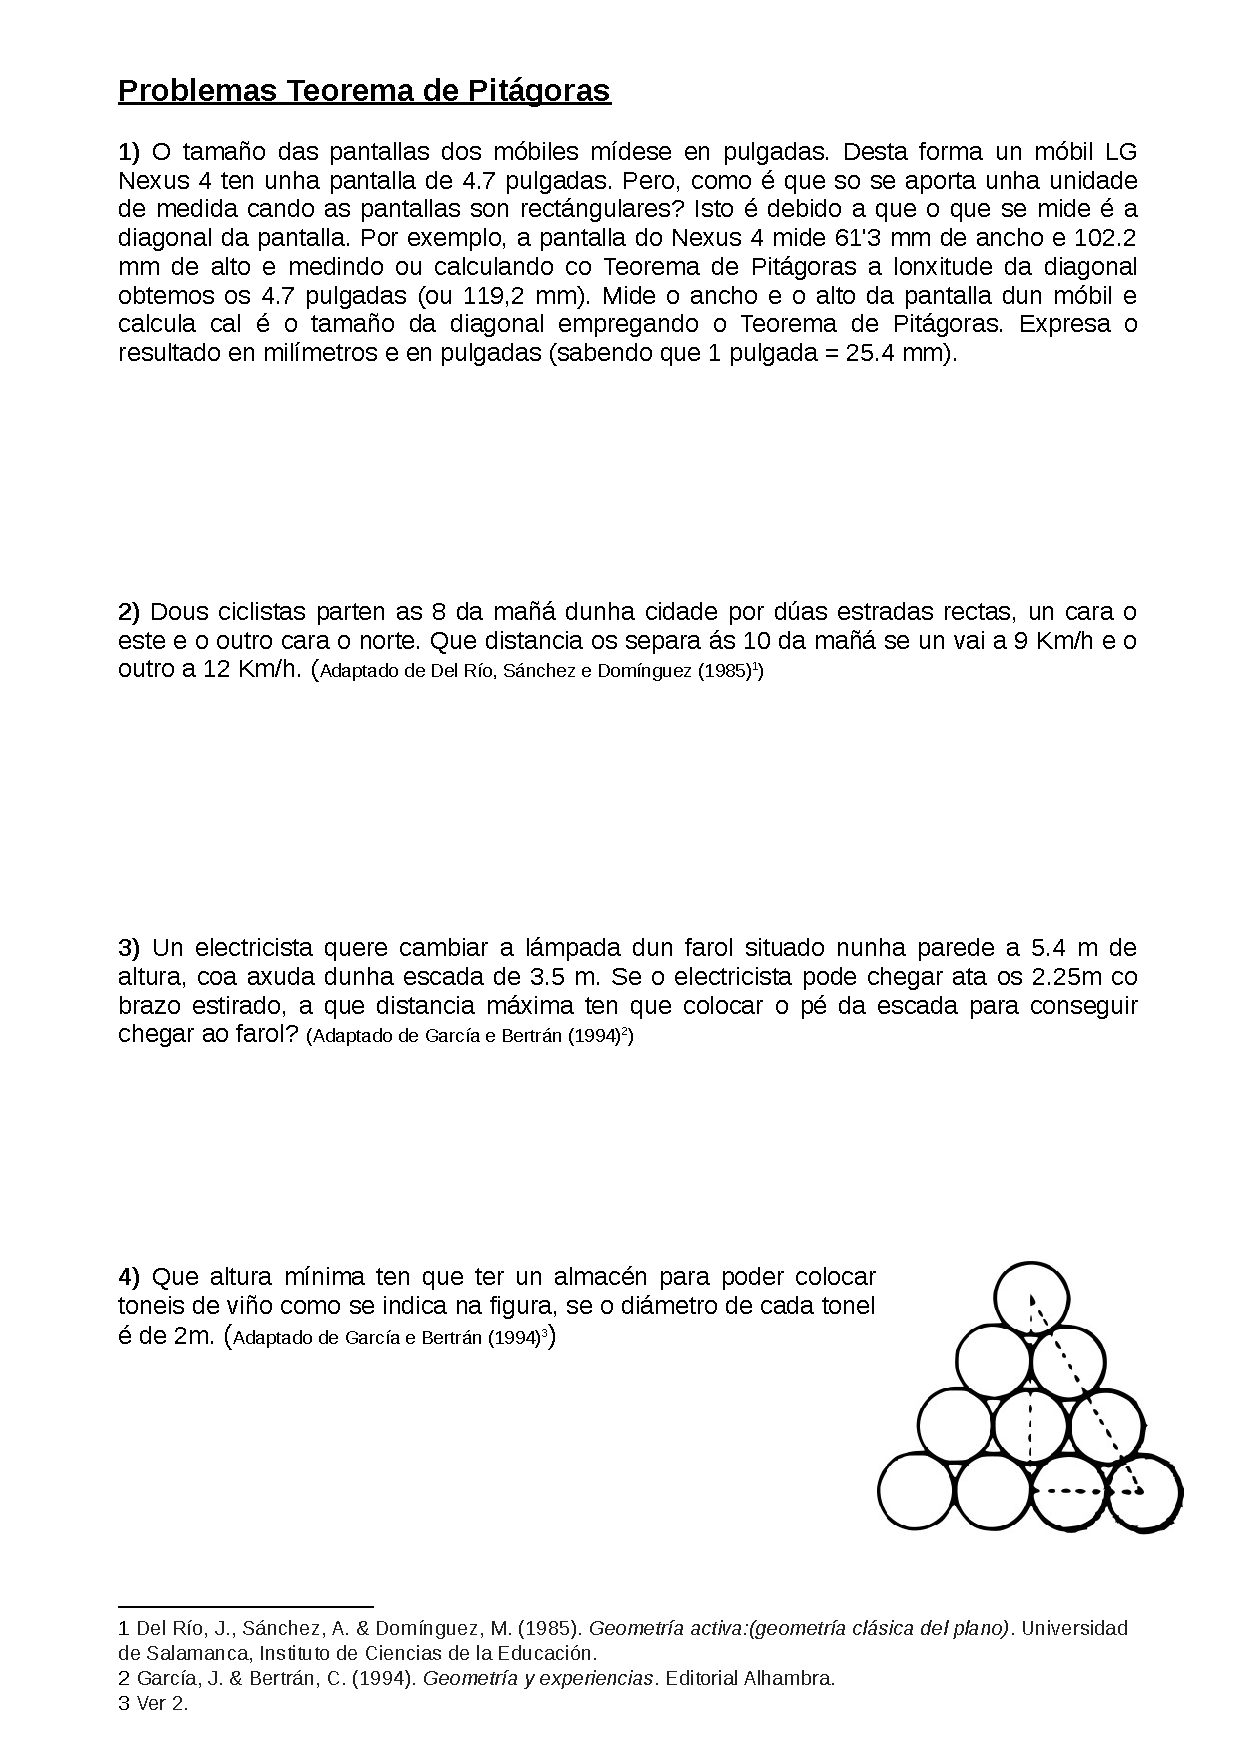
\includepdf[pages=1,scale=0.8,offset=0mm -17mm, frame,pagecommand={\section{Problemas propostos do Teorema de Pitágoras}\label{fich:pitagoras}}]{pdf/pitagoras.pdf}

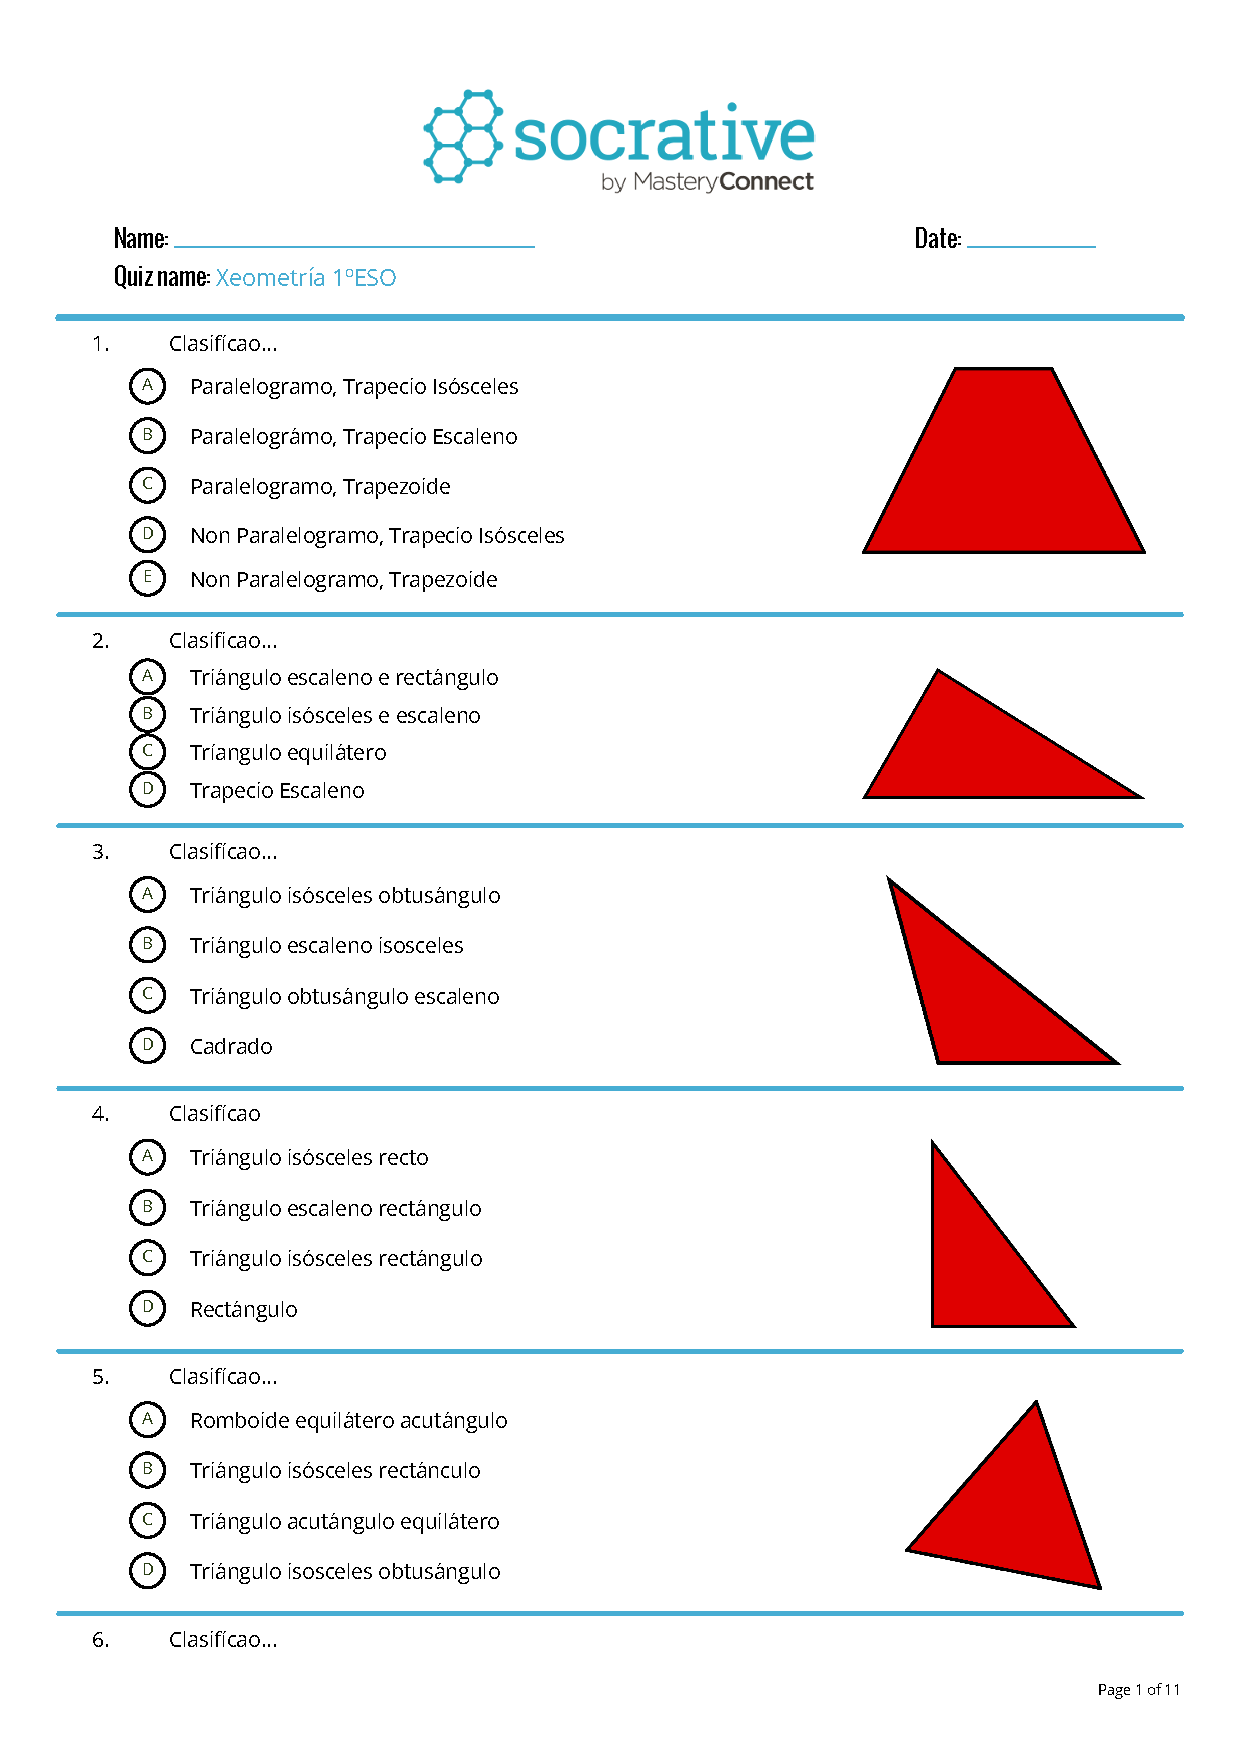
\includepdf[pages=1,scale=0.8,offset=0mm -17mm, frame,pagecommand={\section{Preguntas do Trivial da Actividade 13}\label{fich:trivial}}]{pdf/socrative.pdf}
\includepdf[pages=2-last,scale=0.8,offset=0mm -17mm, frame,pagecommand={}]{pdf/socrative.pdf}

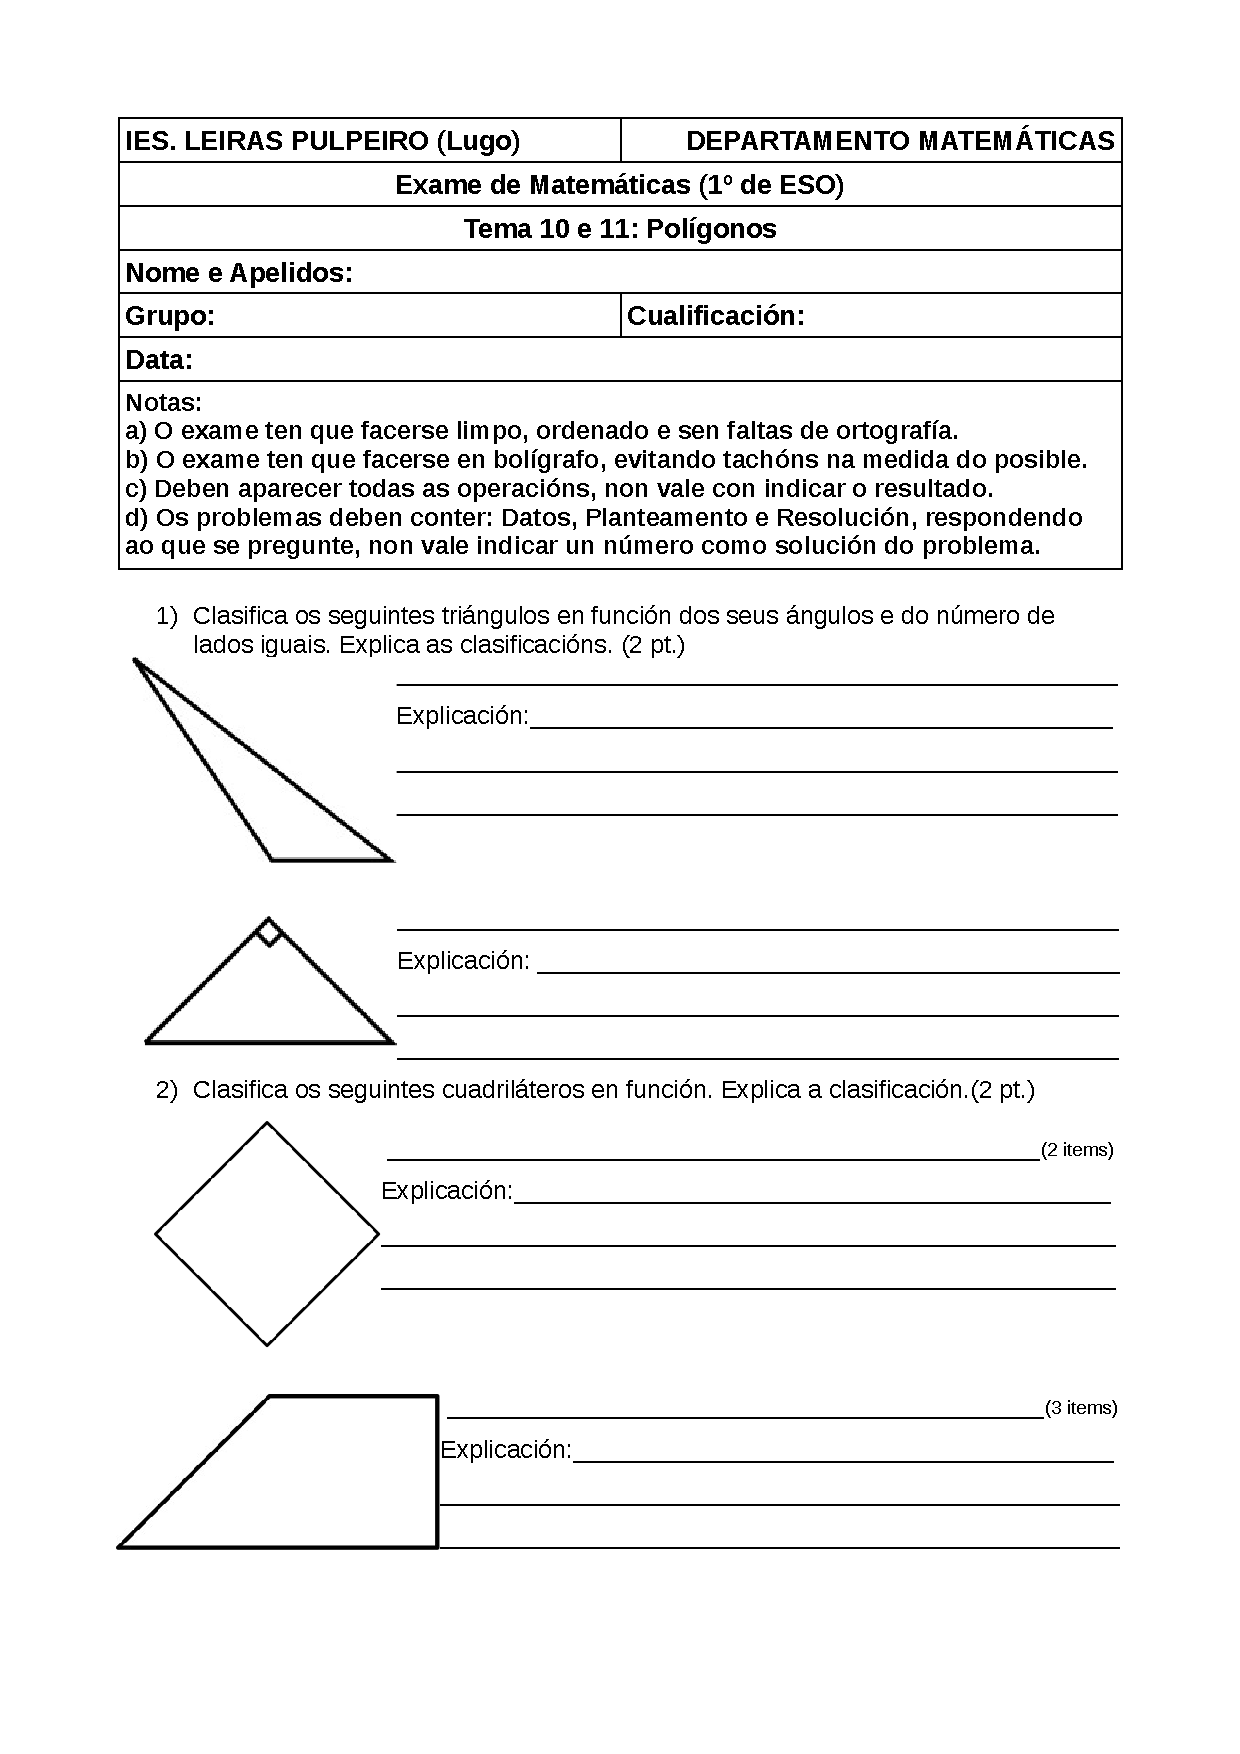
\includepdf[pages=1,scale=0.8,offset=0mm -17mm, frame,pagecommand={\section{Exame Polígonos}\label{fich:ex2}}]{pdf/exame2.pdf}
\includepdf[pages=2,scale=0.8,offset=0mm -17mm, frame,pagecommand={}]{pdf/exame2.pdf}
